\documentclass[tikz]{standalone}
\usetikzlibrary{arrows.meta}
\begin{document}
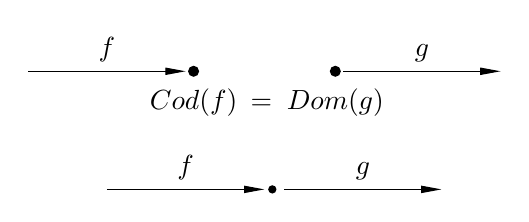
\begin{tikzpicture}[-latex, arrows={-Triangle[angle=20:5pt,scale=1.5]}]
	\draw (0,0) -- node[above] {\(f\)} (2,0);
	\draw (4,0) -- node[above] {\(g\)} (6,0);
	\fill (2.1,0) circle (2pt) node [below=1mm] {\(Cod(f)\)};
	\node at (2.96,-0.42) {\(=\)};
	\fill (3.9,0) circle (2pt) node [below=1mm] {\(Dom(g)\)};
	\draw (1,-1.5) -- node [above] {\(f\)} (3,-1.5);
	\fill (3.1,-1.5) circle (1.5pt);
	\draw (3.25,-1.5) -- node [above] {\(g\)} (5.25,-1.5);
\end{tikzpicture}
\end{document}
